\section{Enclave Operation}

SGX provides trustring computing by protecting the privacy and integrity of the
computation that is performed inside an enclave, and by providing remote
attestation identifying the software running inside an enclavee. This section
describes the processes used to set up an enclave and perform computation
inside it.


\subsection{The Enclave Lifecycle}
\label{sec:lifecycle}

An enclave's lifecycle is deeply intertwined with resource management,
specifically the allocation of EPC pages. Therefore, the instructions that
transition between different lifecycle states can only be executed by
privileged software, such as an OS kernel or hypervisor. Enclaves go through
the following phases.

% ECREATE, EADD, EREMOVE: SGX/SGX2 S 5.3

\textbf{Creation.} An enclave is born when privileged software issues the
ECREATE instruction to create a SECS page (\S~\ref{sec:secs}). Most
importantly, ECREATE establishes the enclave's identity, represented by a
64-bit enclave ID, which is used to keep track of the enclave's pages in the
EPCM.

\textbf{Setup.} ECREATE marks the newly created SECS as \textit{uninitialized}.
In this state, privileged software issues EADD instructions that build up the
enclave's initial state. This includes creating TCS pages (\S~\ref{sec:tcs})
and regular pages that hold the SSA sequences referenced by TCS pages, as well
as the enclave's code and data. EADD requires a reference to the SECS of the
enclave that will own the newly allocated EPC page, and
refuses\footnote{results in a General Protection fault (\#GP)} to operate if
the SECS is in the initialized state.

\textbf{Launch.} After building up the enclave's initial state, privileged
software follows a largely undocumented process that ends with the execution of
an EINIT instruction, which marks the enclave's SECS as \textit{initialized}.
The undocumented process revolves around obtaining permission to launch the
enclave, which is expressed in the EINITTOKEN data structure. We present more
information about the launch process in \S~TODO.

\textbf{Execution.} While an enclave is initialized, it can perform computation
in the isolated environment that provides the SGX security guarantees. When
executing an enclave's code, a logical processor is in \textit{enclave mode},
which is explained in detail in \S~\ref{sec:enclave_mode} below.

\textbf{Teardown.} After the enclave has done the computation it was designed
to perform, privileged code executes the EREMOVE instructions to deallocate its
EPC pages.

\begin{figure}[hbt]
  \center{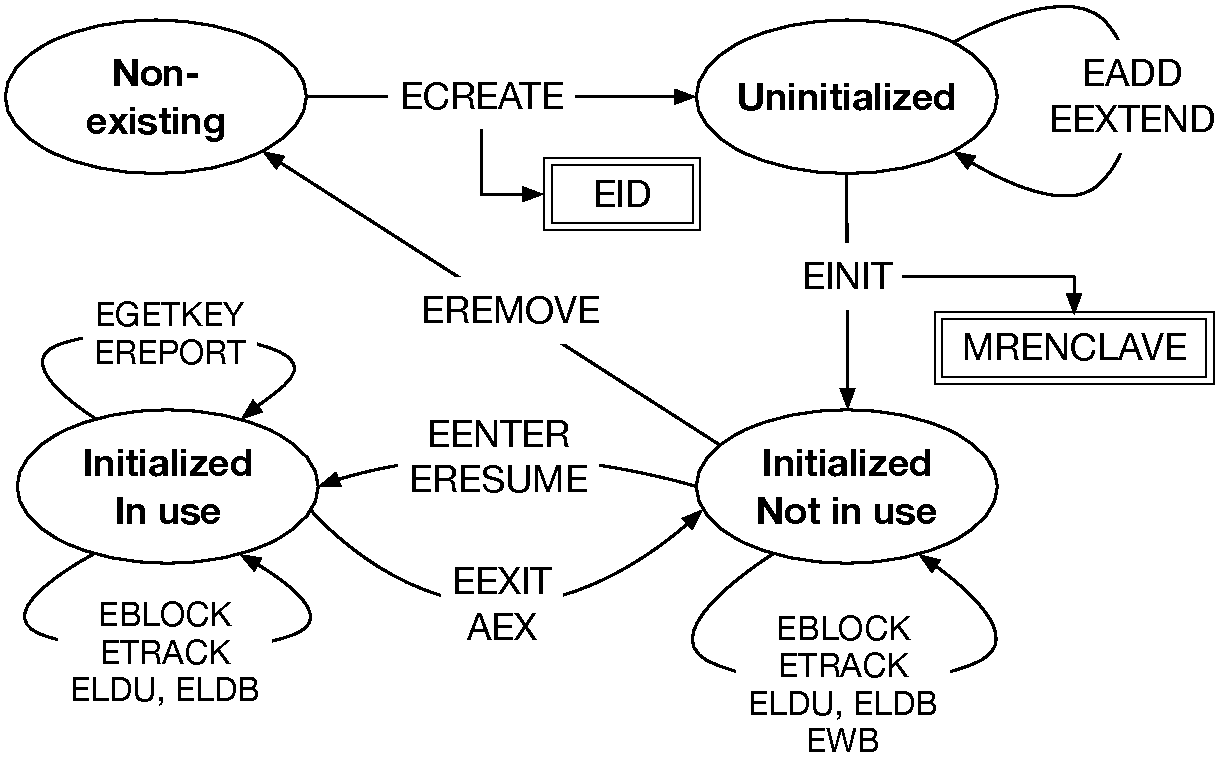
\includegraphics[width=85mm]{figures/enclave_lifecycle.pdf}}
  \caption{
    The SGX enclave lifecycle management instructions and state transition.
    ECREATE establishes the enclave's ID (EID). EINIT sets MRENCLAVE, the
    enclave setup hash certified by the attestation process.
  }
  \label{fig:enclave_lifecycle}
\end{figure}


\subsection{The Enclave Mode}
\label{sec:enclave_mode}

% Internal CREGs: SGX/SGX2 S 5.1.4
% Access Control Requirements: SGX/SGX2 S 2.3

When executing the code inside an enclave, a logical processor is said to be
\textit{in enclave mode}. When a processor is outside enclave mode, software
cannot access any memory inside the PRM range. In enclave mode, the CPU allows
accesses to EPC pages that belong to the currently executing enclave.

Assuming no interrupts or faults, a logical processor transitions into enclave
mode by executes the EENTER instruction. EENTER can only be executed by
unprivileged software (running at ring 3), because SGX was designed to be used
by user-level programs. EENTER can only be used to jump into pre-defined
locations inside an enclave, for the same reasons that system calls only jump
at specific locations in an OS kernel. When all the preconditions (described
below) are met, EENTER causes the logical processor to enter enclave mode, and
keeps it at ring 3.

SGX restricts enclaves to ring 3, maintaining the roles of the OS kernel and
hypervisor as resource managers. This makes it possible for an infrastructure
owner to allow user-supplied software to create and use enclaves, while having
the assurance that the OS kernel and hypervisor can still protect the
infrastructure from buggy or malicious software.




\subsubsection{Interrupt / Fault Handling}
\label{sec:aex}





\subsection{Evicting EPC Pages}
\label{sec:sgx_ewb}

% Eviction of Enclave Pages: SGX S 3.5.3

% EPA: SGX S 5.3 EPA

\begin{figure}[hbt!]
  \center{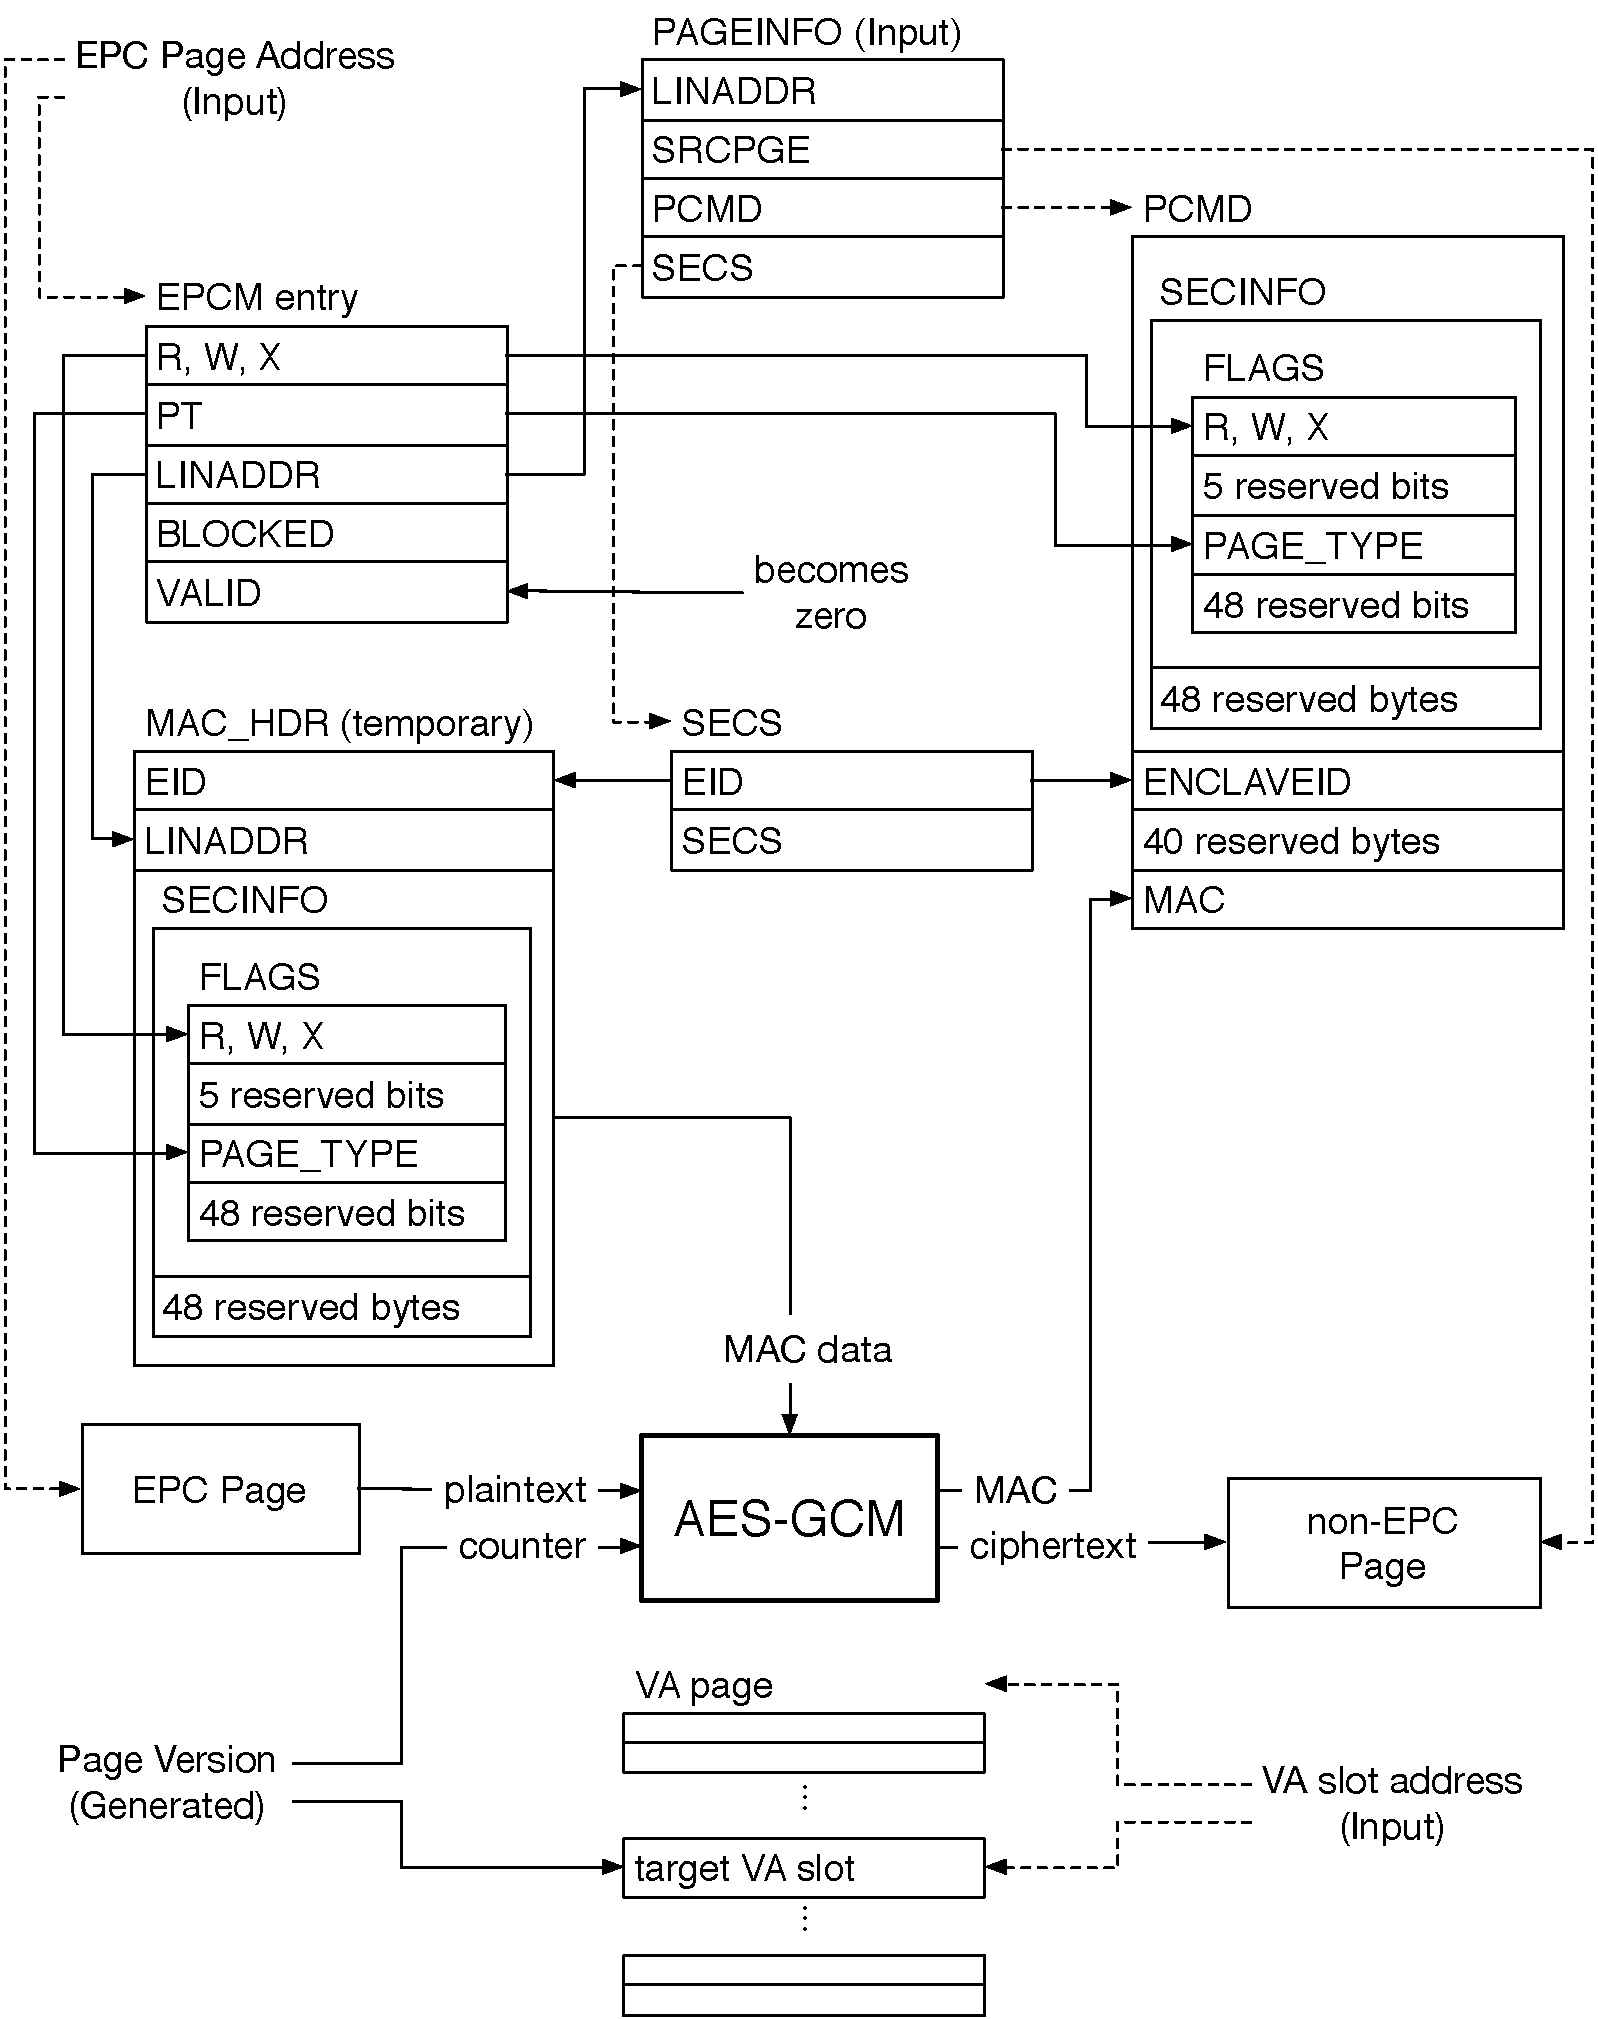
\includegraphics[width=85mm]{figures/sgx_ewb.pdf}}
  \caption{
    The data flow of the EWB instruction that evicts an EPC page. The page's
    content is encrypted in a non-EPC RAM page. A nonce is created and saved
    in an empty slot inside a VA page. The page's EPCM metadata and a MAC
    are saved in a separate area in non-EPC memory.
  }
  \label{fig:sgx_ewb}
\end{figure}

% Loading an Enclave Page: SGX S 3.5.4

